\begin{appendices}
%Appendix A
\chapter{X-ray spectral modelling plots}
\label{Appendix_Xray_spectra}
%First Figure
\begin{figure}[h]
\begin{subfigure}{\textwidth}
	\centering
	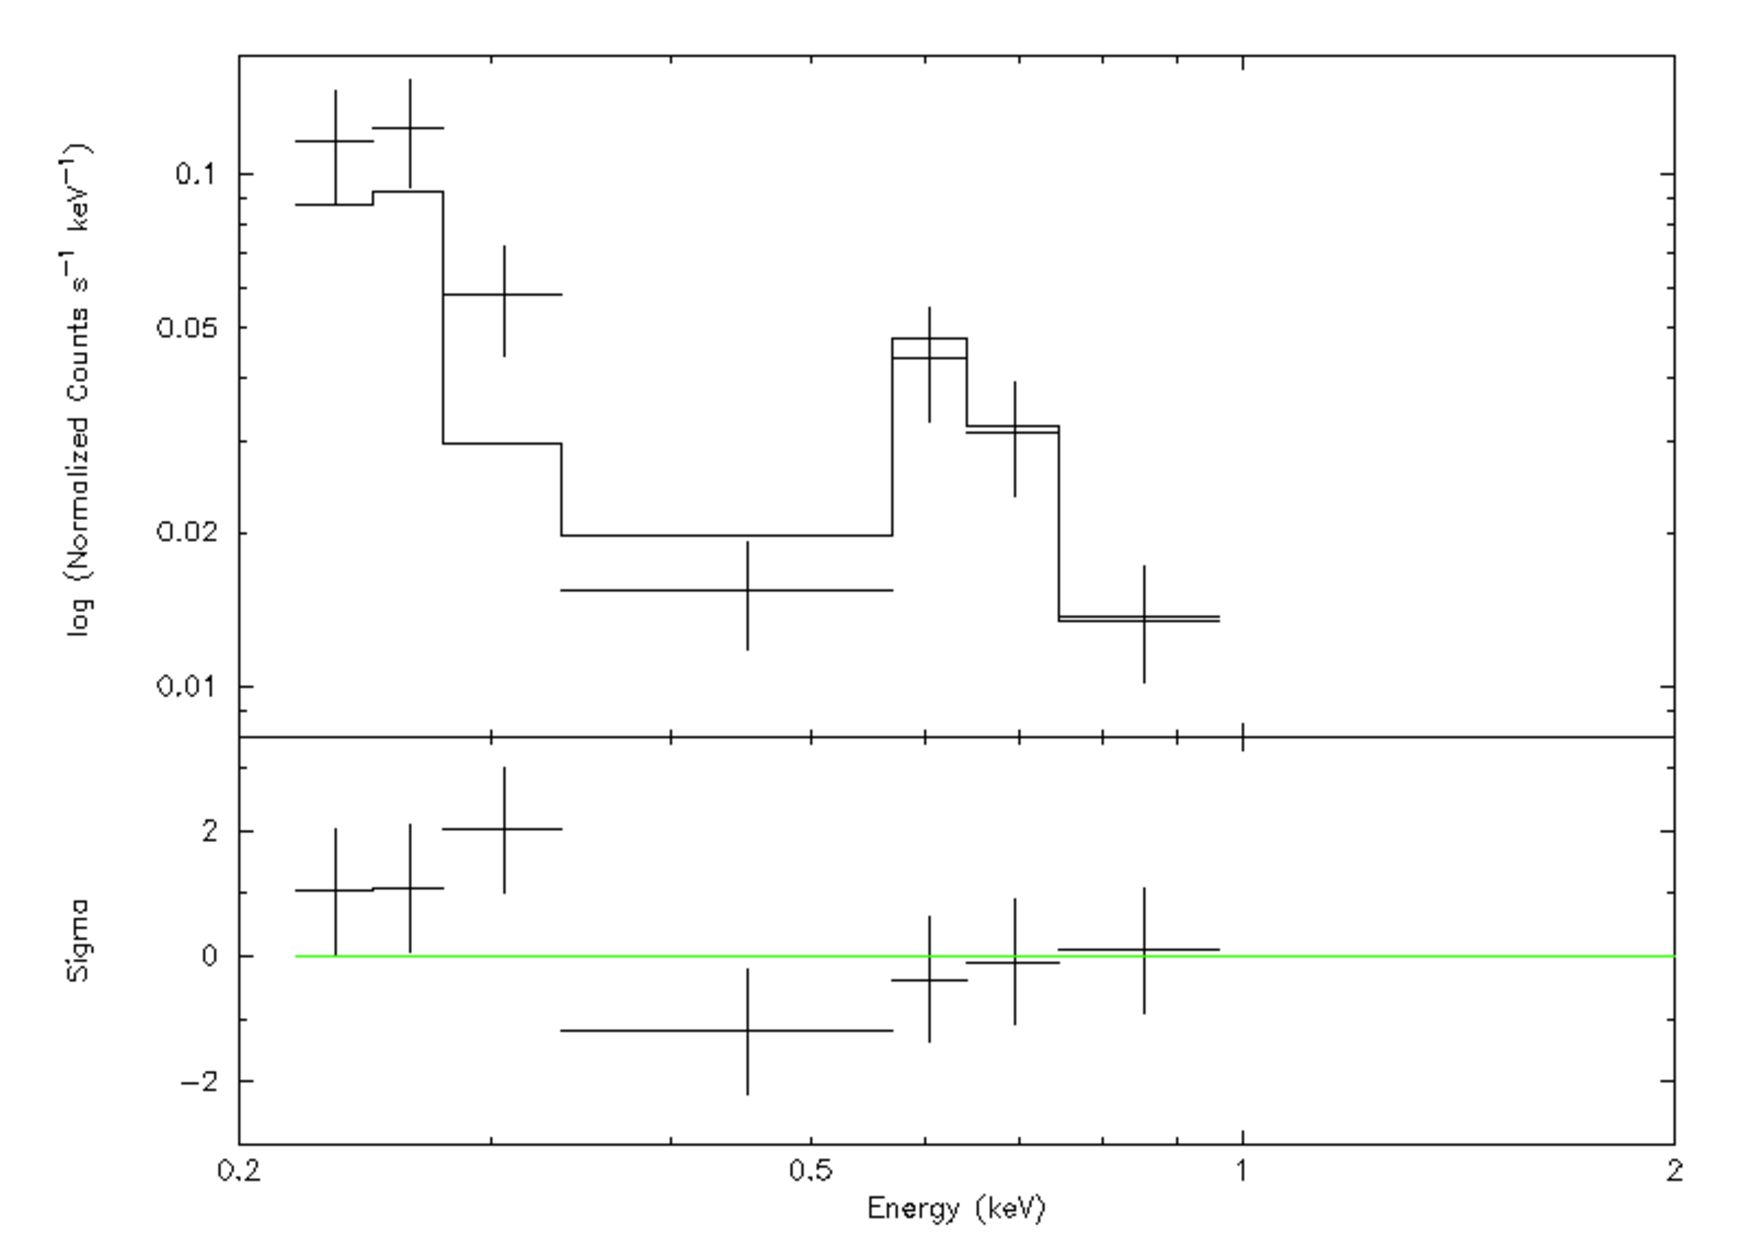
\includegraphics[height = 0.23\paperheight,width=0.9\textwidth]{Figures/3-Xray_age/spec_40eria}
	\caption{40 Eri A}
\end{subfigure}
\begin{subfigure}{\textwidth}
	\centering
	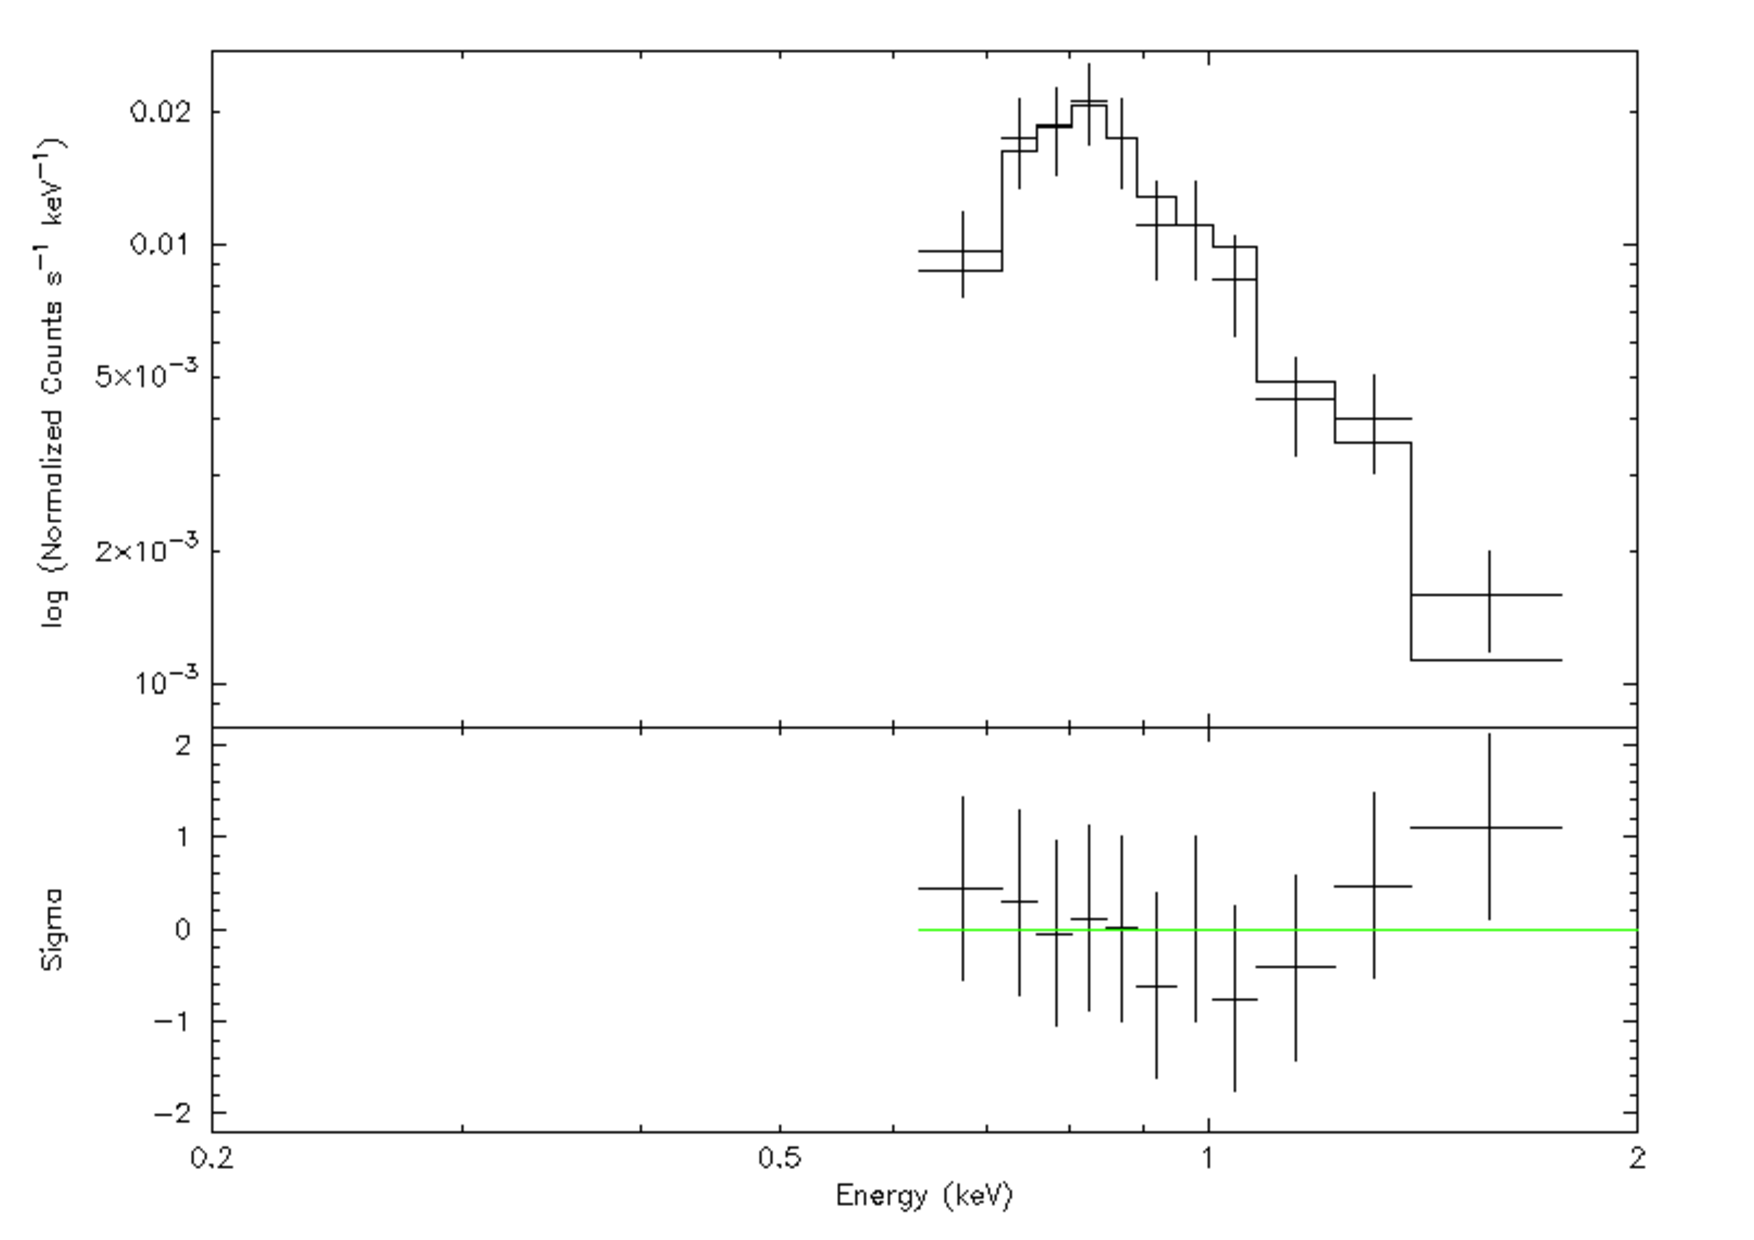
\includegraphics[height = 0.23\paperheight,width=0.9\textwidth]{Figures/3-Xray_age/spec_cd-3710500}
	\caption{CD -3710500}
\end{subfigure}

\caption[X-ray spectra of 40 Eri A and CD -3710500]{X-ray spectra (grouped to 15 counts per bin) and best fit models of two X-ray sources. The top region of each subplot shows the number of counts per second per keV as a function of energy. The bottom region of each subplot shows the sigma value for the best fit model as a function of energy. CD -3710500 was observed with a front-illuminated \textit{Chandra} CCD and therefore only has spectral data above 0.6 keV.}
\label{App_A_40EriA_CD3710500}
\end{figure}

%Second Figure
\begin{figure*}
\begin{subfigure}{\textwidth}
	\centering
	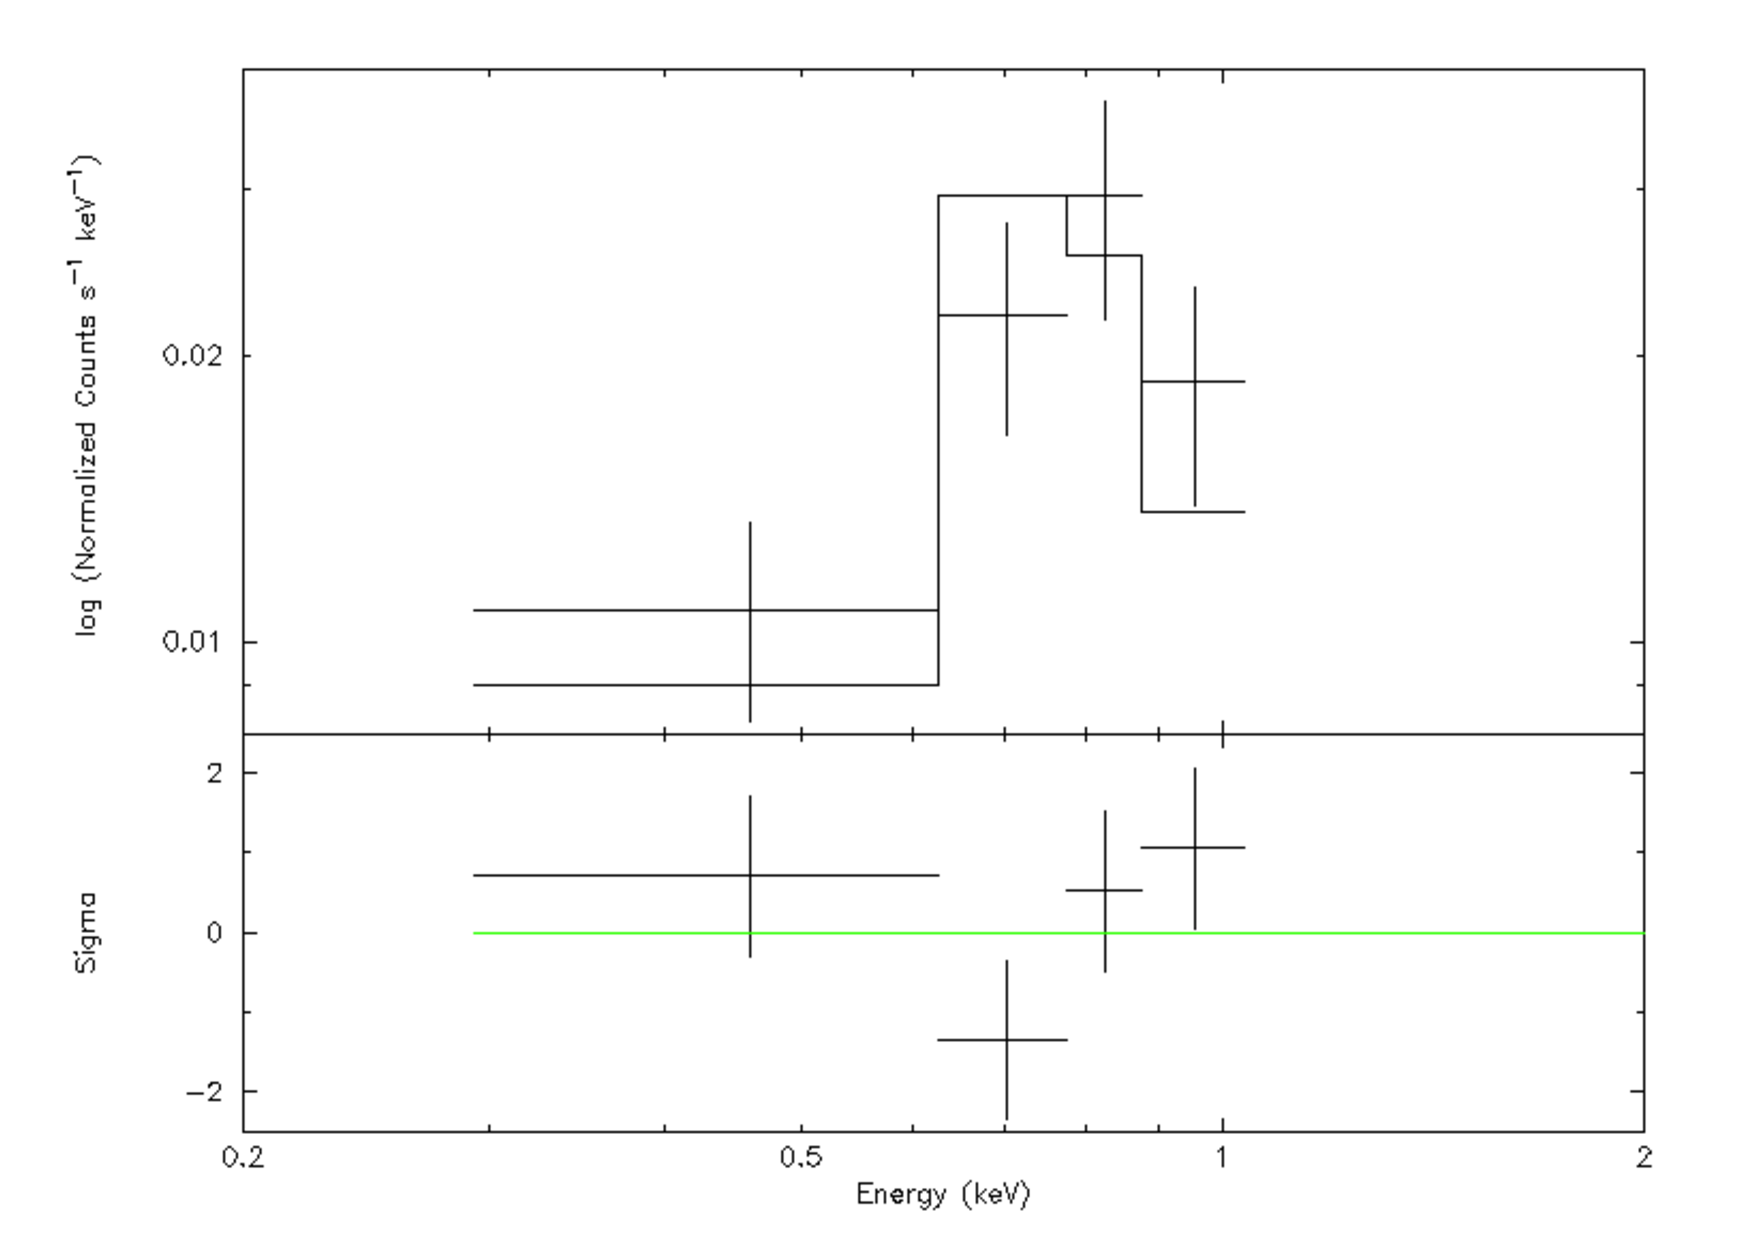
\includegraphics[height = 0.25\paperheight,width=\textwidth]{Figures/3-Xray_age/spec_gj176}
	\caption{GJ 176}
\end{subfigure}
\begin{subfigure}{\textwidth}
	\centering
	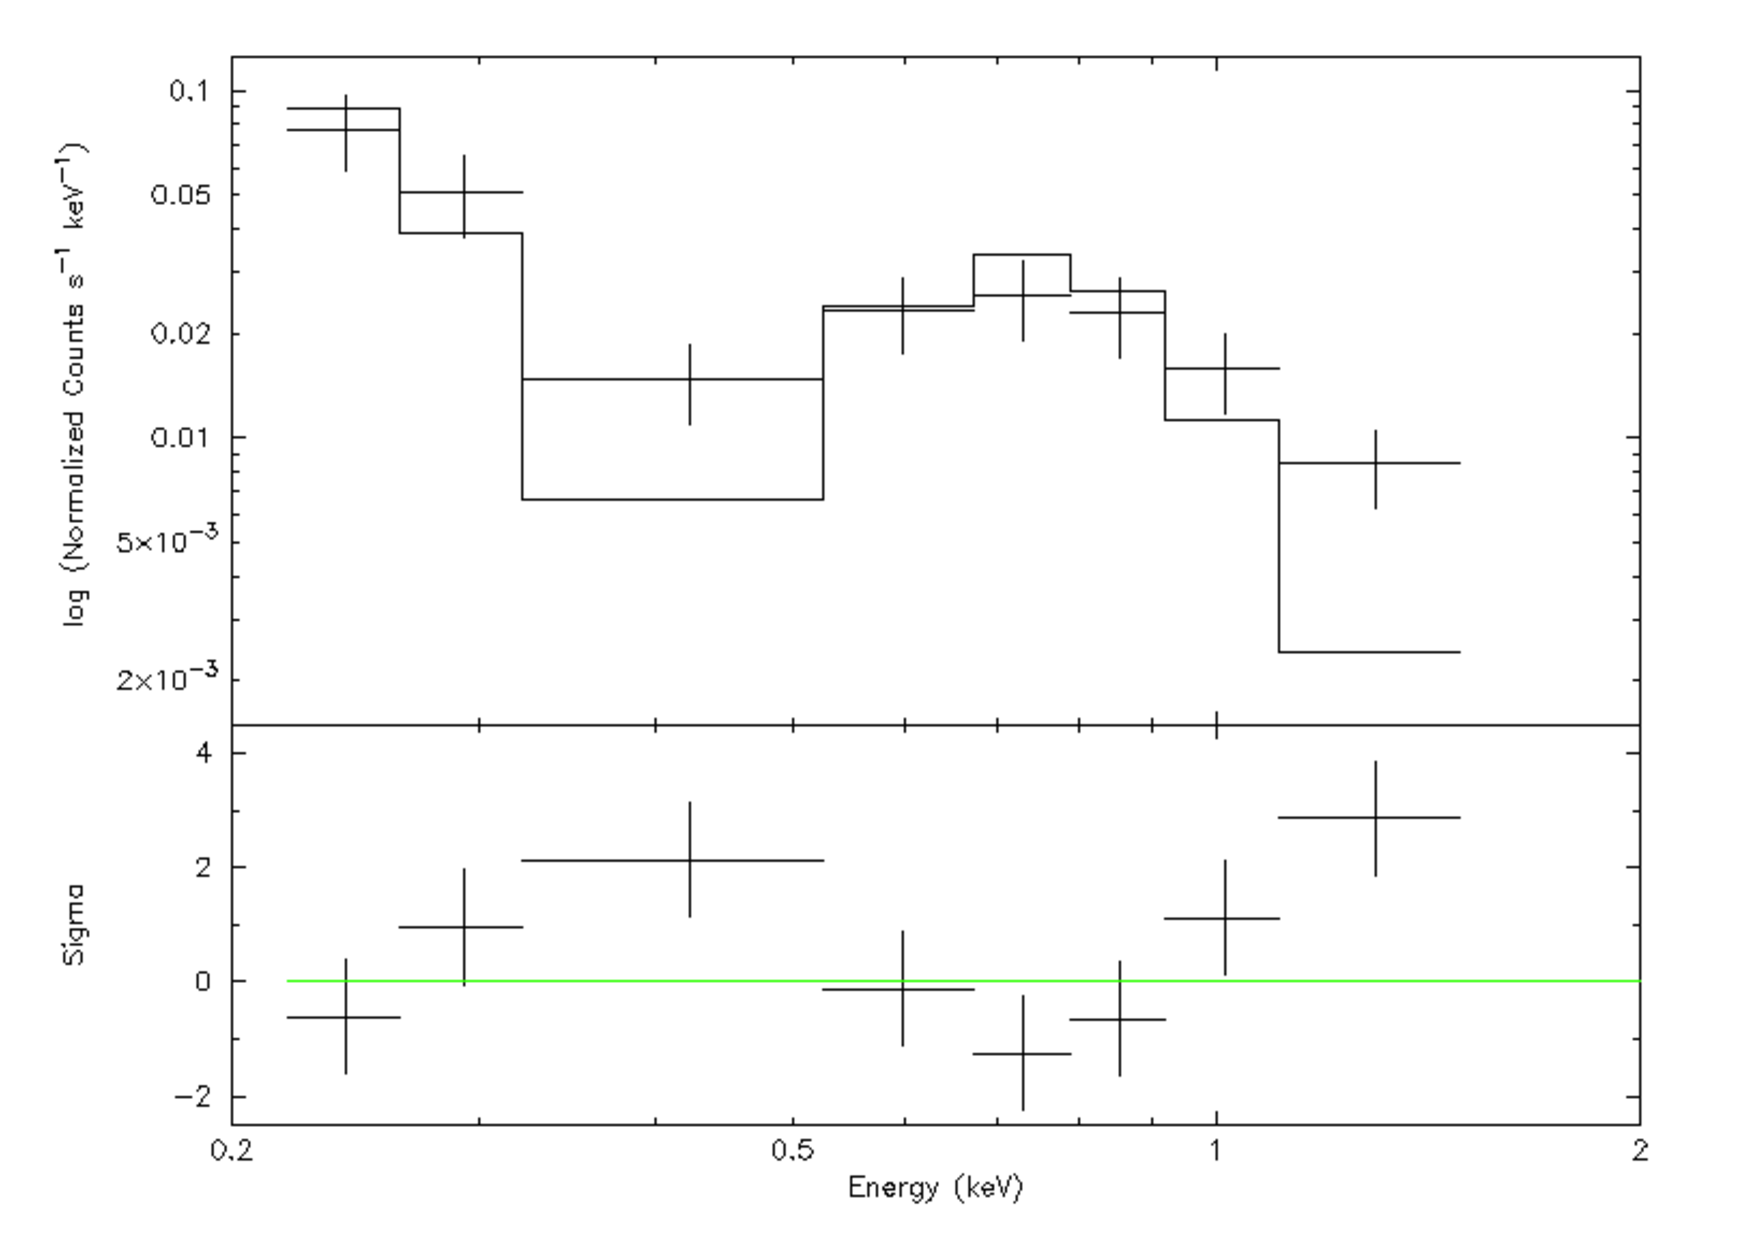
\includegraphics[height = 0.25\paperheight,width=\textwidth]{Figures/3-Xray_age/spec_gj191}
	\caption{GJ 191}
\end{subfigure}

\caption[X-ray spectra of GJ 176 and GJ 191]{X-ray spectra (grouped to 15 counts per bin) and best fit models of two X-ray sources. The top region of each subplot shows the number of counts per second per keV as a function of energy. The bottom region of each subplot shows the sigma value for the best fit model as a function of energy.}
\label{App_A_GJ176_GJ191}
\end{figure*}


%Third Figure
\begin{figure*}
\begin{subfigure}{\textwidth}
	\centering
	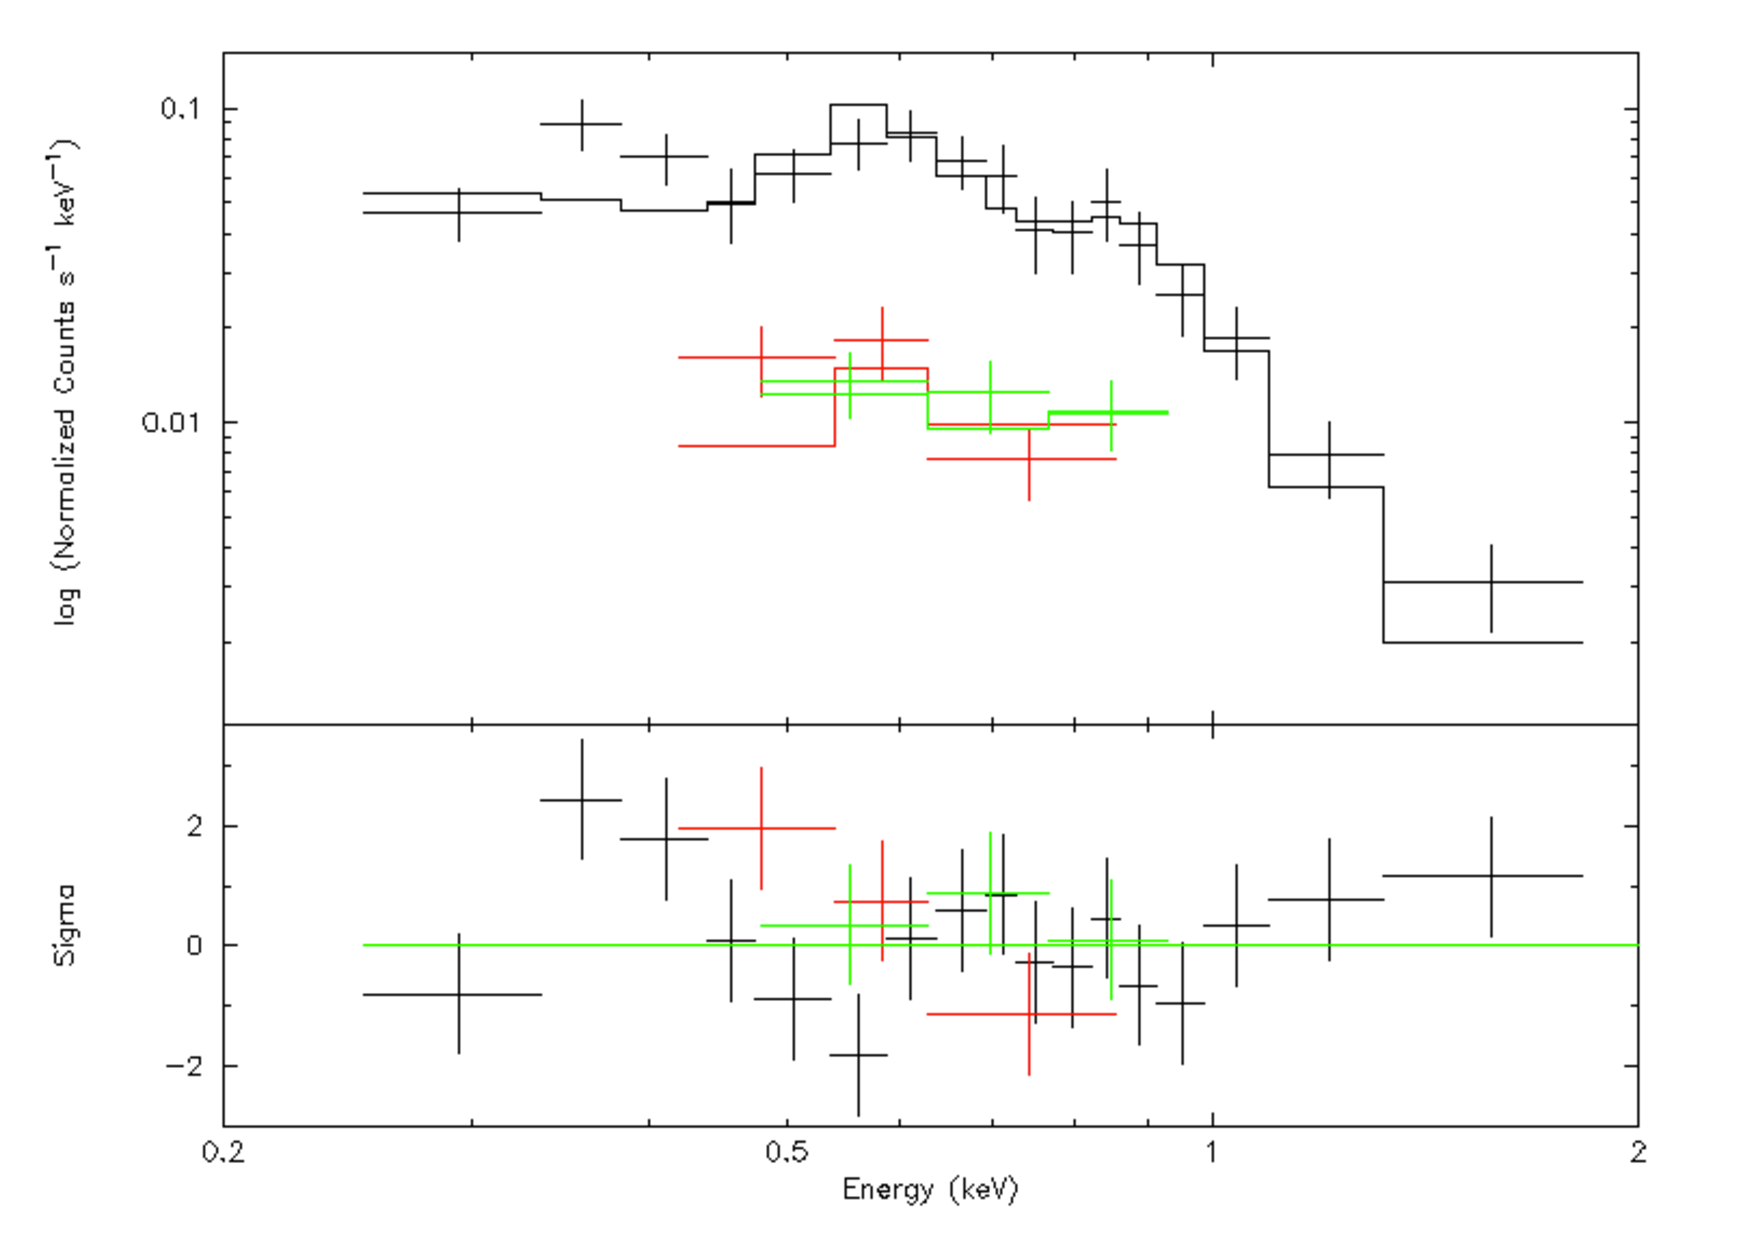
\includegraphics[height = 0.25\paperheight,width=\textwidth]{Figures/3-Xray_age/spec_hr7703}
	\caption{HR 7703}
\end{subfigure}
\begin{subfigure}{\textwidth}
	\centering
	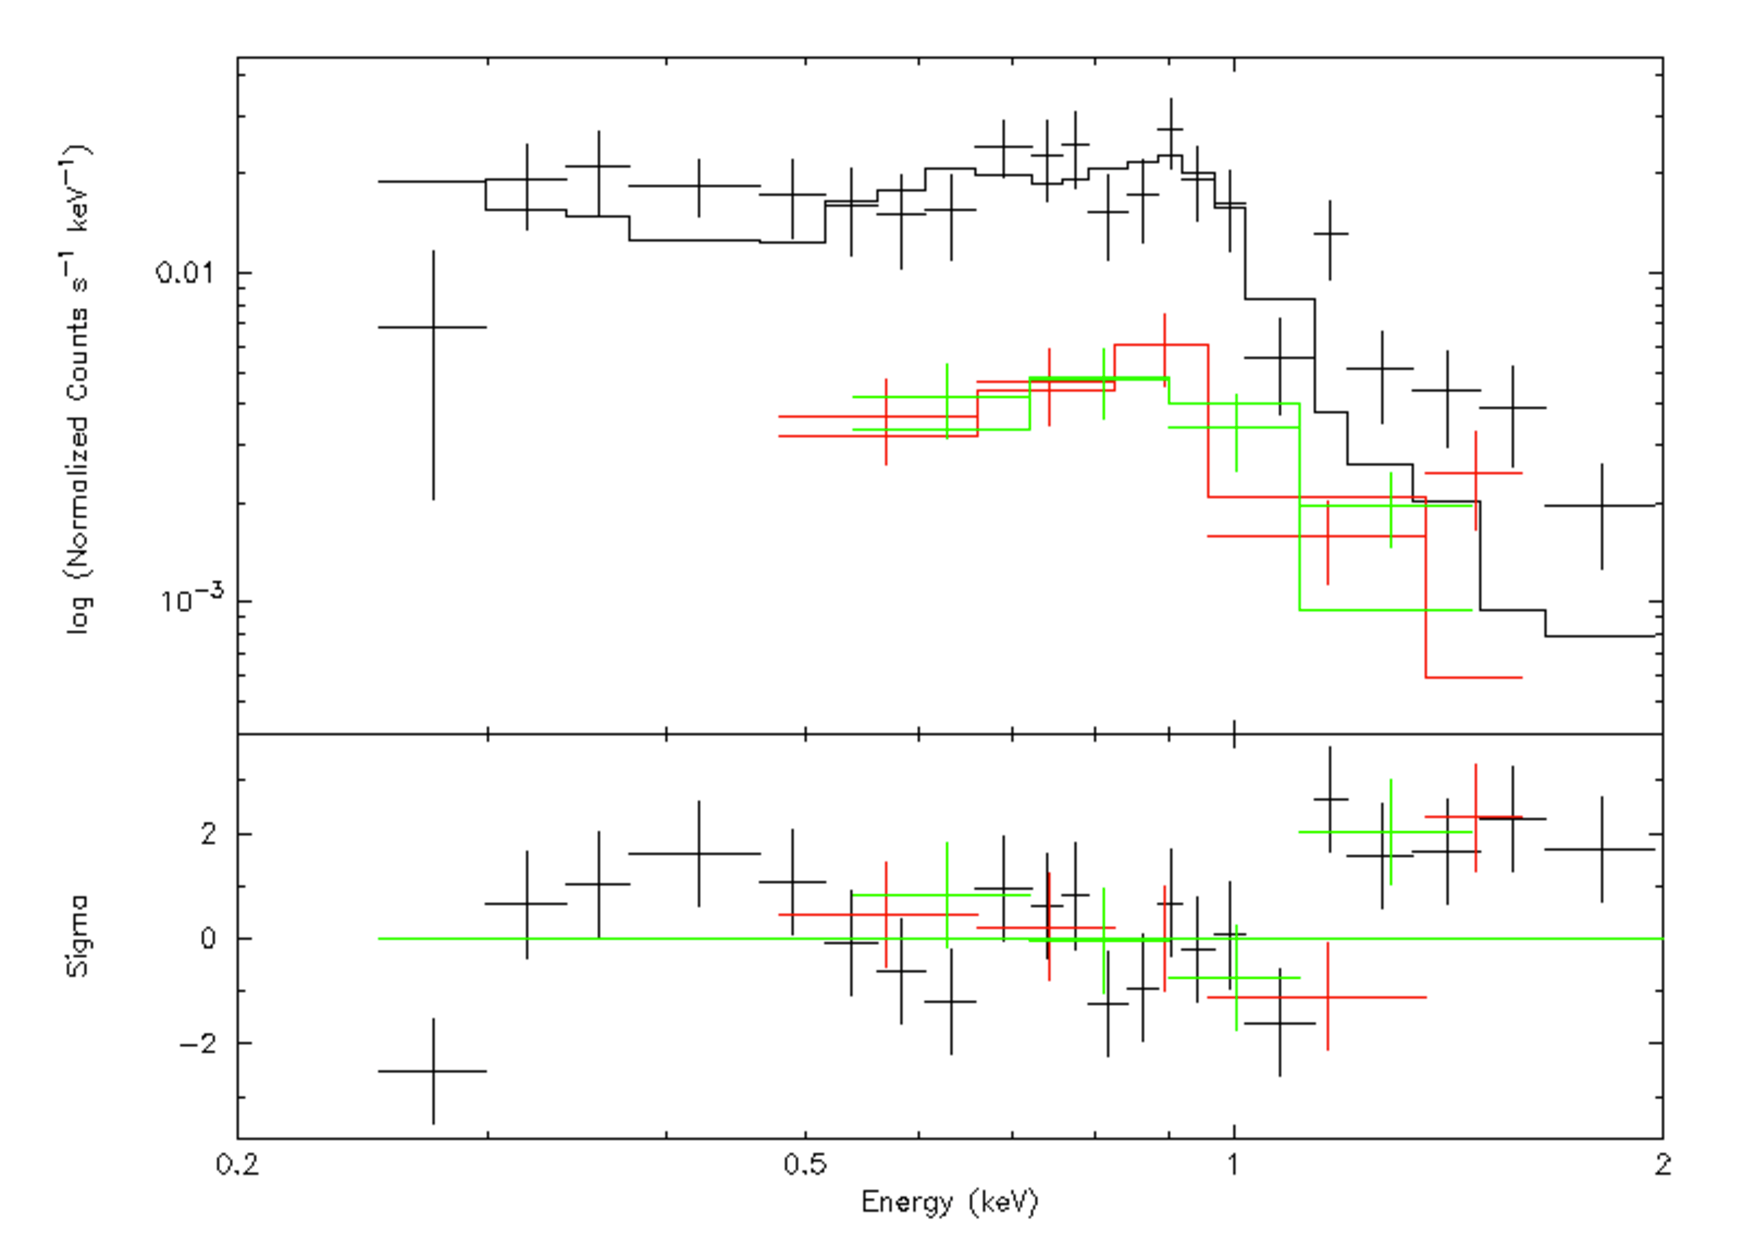
\includegraphics[height = 0.25\paperheight,width=\textwidth]{Figures/3-Xray_age/spec_kic7529180}
	\caption{KIC 7529180}
\end{subfigure}

\caption[X-ray spectra of HR 7703 and KIC 7529180]{X-ray spectra (grouped to 15 counts per bin) and best fit models of two X-ray sources. The top region of each subplot shows the number of counts per second per keV as a function of energy. The bottom region of each subplot shows the sigma value for the best fit model as a function of energy. Different colours indicate spectra from different detectors which are fitted simultaneously to ensure a more accurate fit.}
\label{App_A_HR7703_KIC7529180}
\end{figure*}

%Fourth Figure
\begin{figure*}
\begin{subfigure}{\textwidth}
	\centering
	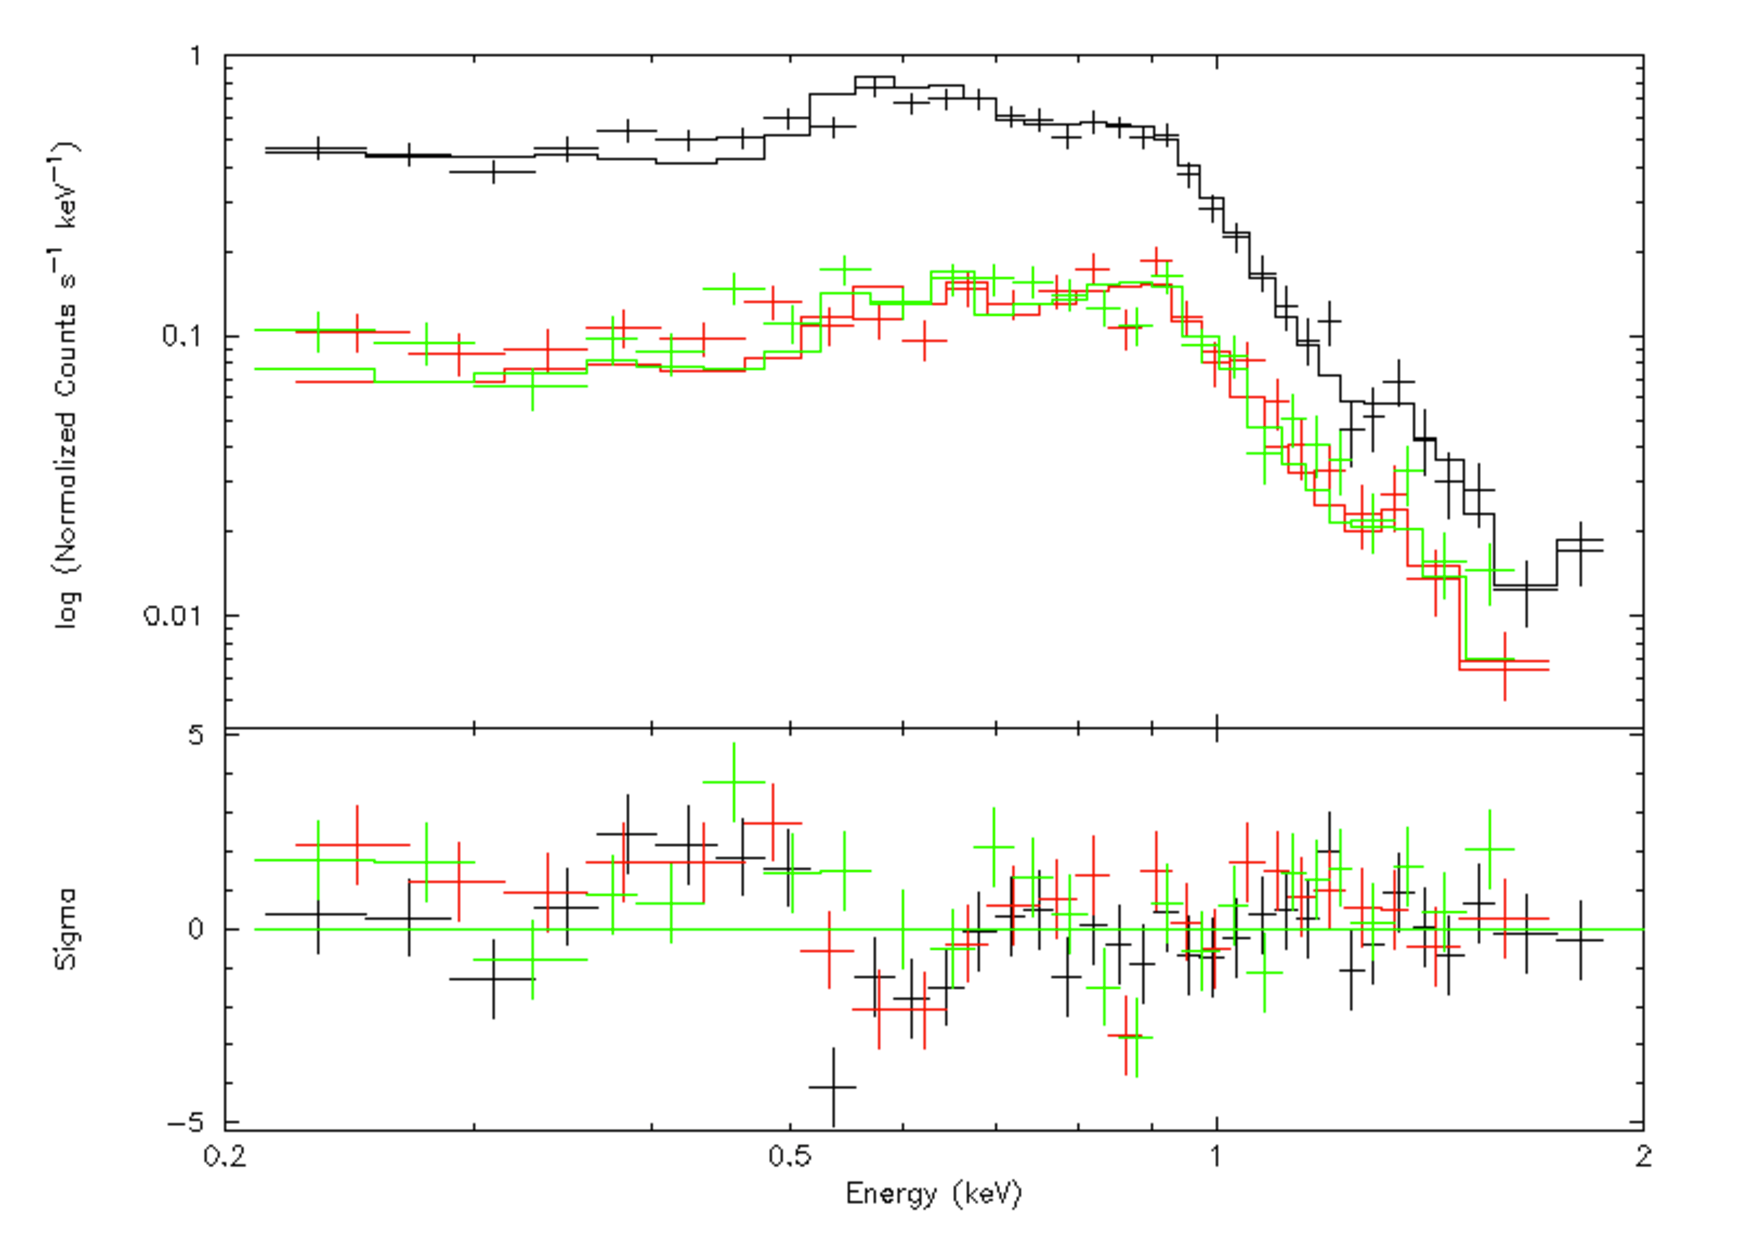
\includegraphics[height = 0.25\paperheight,width=\textwidth]{Figures/3-Xray_age/spec_61cyga}
	\caption{61 Cyg A}
\end{subfigure}
\begin{subfigure}{\textwidth}
\centering
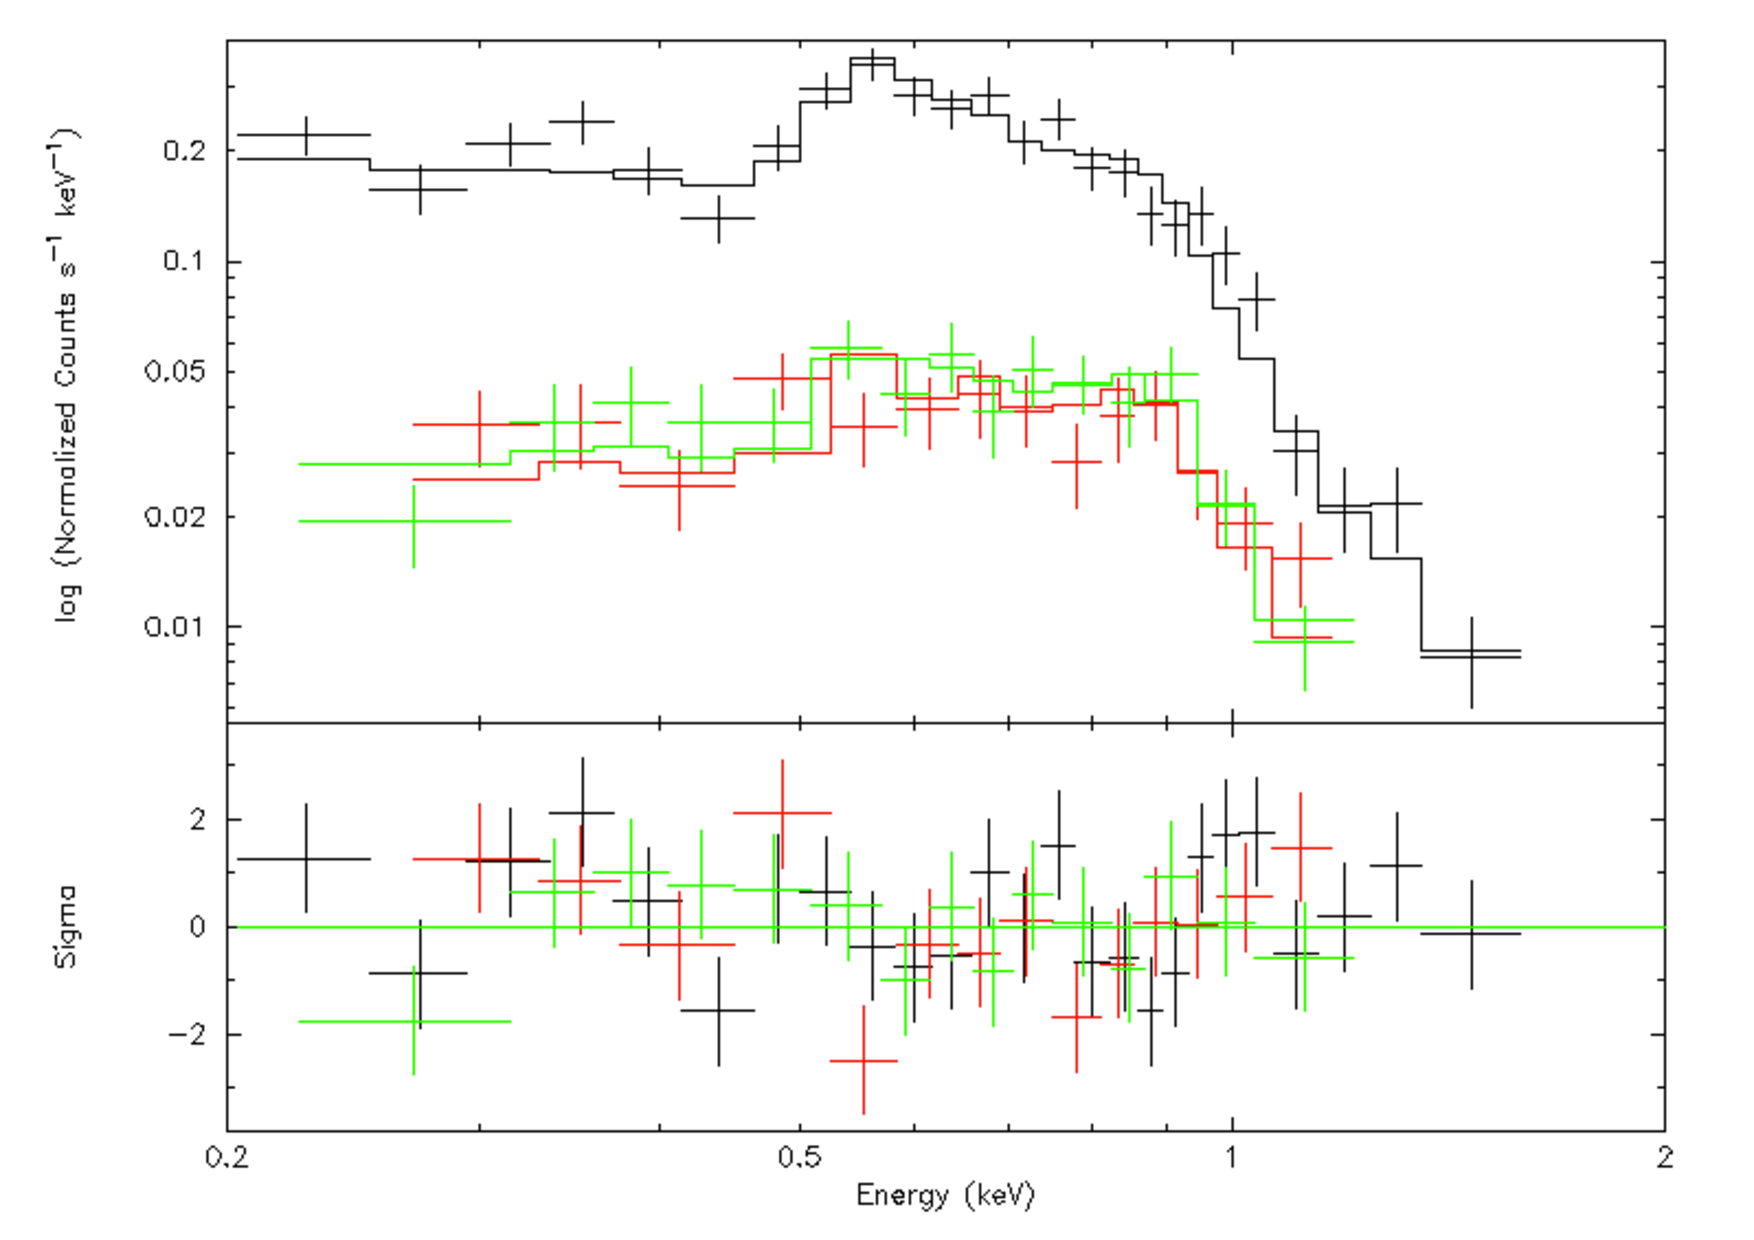
\includegraphics[height =        0.25\paperheight,width=\textwidth]{Figures/3-Xray_age/spec_61cygb}
\caption{61 Cyg B}
\end{subfigure}
\par\bigskip

\caption[X-ray spectra of 61 Cyg A and B]{X-ray spectra (grouped to 15 counts per bin) and best fit models for one exemplary observation of 61 Cyg A and B, respectively. These sources were detected to at least three sigma and contained over a hundred counts in the source region. The top region of each subplot shows the number of counts per second per keV as a function of energy. The bottom region of each subplot shows the sigma value for the best fit model as a function of energy. Different colours indicate spectra from different detectors which are fitted simultaneously to ensure a more accurate fit.}
\label{App_A_61Cyg}
\end{figure*}










\chapter{testing 2}
\end{appendices}